%TODO keine jahresangaben, con vs prob andere Farben, Wenn conjugacy raus, dann kein k(G) mehr
\documentclass[11ptt,english,usepdftitle=false,leqno]{beamer}%,dvips,xcolor=pst  pdfpagelabels=false,,handout
\hypersetup{pdfpagemode=FullScreen,pdftitle={Things left to prove}} %,pdfstartview={}
\usepackage{babel}
\usepackage[utf8]{inputenc}
\usepackage[T1]{fontenc}
%\usepackage{appendixnumberbeamer}
\usepackage{enumerate}
\usepackage{amsmath} %amssymb
%\usepackage{pifont}
%\usepackage{booktabs}
\usepackage{thmtools}
%\usepackage{xparse}
%\usepackage{pgf}
%\usepackage{graphicx}
%\usepackage{epstopdf}
\usepackage{tikz}
%\usepackage{tikzsymbols,tikz-cd}
\usetikzlibrary{calc}
\usetikzlibrary{positioning}
%\usetikzlibrary{decorations.pathmorphing,overlay-beamer-styles}
%\definecolor{paper}{RGB}{239,227,157}
\let\Tiny=\tiny
\renewcommand{\raggedright}{\leftskip=0pt \rightskip=0pt plus 0cm}
%\usetheme{default}
\usetheme{Boadilla}
\usefonttheme[onlymath]{serif}
\setbeamertemplate{enumerate items}[circle]
%\setbeamercolor{title}{bg=white} %fg=black, 
%\setbeamercolor{subtitle}{fg=black}

\addtobeamertemplate{headline}{%
  \leavevmode%
  \hbox{%
  \begin{beamercolorbox}[wd=\paperwidth,ht=2.25ex,dp=1ex,center]{author in head/foot}%
     \insertsectionnavigationhorizontal{\paperwidth}{}{}
  \end{beamercolorbox}}%
}

%\setbeamertemplate{title}{
%  \centering
%  \usebeamerfont{title}\usebeamercolor[fg]{title}%
%  \fbox{\parbox{5cm}{\centering\insertshorttitle}}
%}

%\setbeamercolor{normal}{bg=white,fg=black}
%\pgfsetfillopacity{0.5}
%\begin{beamercolorbox}[wd=3cm]{normal}
%
%\end{beamercolorbox}
%\pgfsetfillopacity{1}

\title[Things left to prove]{Things left to prove}
\author{Benjamin Sambale}%\vspace{2cm}\\
\subtitle{Characters and Blocks of Finite Groups\\Gabriel's conference 2025}
%\institute[LUH]{Leibniz Universität Hannover}
\date{31th January 2025}

%\newTheorem*{Thm}{Theorem}
%\newTheorem*{Prop}{Proposition}
%\newTheorem*{Cor}{Corollary}
%\newTheorem*{Con}{Conjecture}
%\newcommand{Prop}{\begin{alertblock}{Problem}
\renewenvironment{problem}[1][\unskip]{%
	\setbeamercolor{block title}{fg=black, bg=yellow, }
  \setbeamercolor{block body}{fg=black, bg=yellow!30}
  \begin{block}{Problem #1}}{\end{block}}
%\newenvironment{Prob}[1][\unskip]{\begin{problem}{Problem #1}}{\end{problem}}
%\setbeamercolor{Theorem}{bg=red!50,fg=black}
\newenvironment{Con}[1][\unskip]{\begin{alertblock}{Conjecture #1}}{\end{alertblock}}
%\newenvironment{sm}{\bigl(\begin{smallmatrix}}{\end{smallmatrix}\bigr)}
%\newTheorem{Prob}{Problem}
%\newenvironment<>{Prob}[1][]{%
%  \setbeamercolor{block title example}{fg=white,bg=red!75!black}%
%  \begin{example}#2[#1]}{\end{example}}

\newcommand{\GL}{\mathrm{GL}}
\newcommand{\Sym}{\mathrm{Sym}}
\newcommand{\Inn}{\mathrm{Inn}}
\newcommand{\PSL}{\mathrm{PSL}}
\newcommand{\Syl}{\mathrm{Syl}}
\newcommand{\Gal}{\mathrm{Gal}}
\newcommand{\Z}{\mathrm{Z}}
\newcommand{\C}{\mathrm{C}}
\newcommand{\N}{\mathrm{N}}
\newcommand{\ZZ}{\mathbb{Z}}
\newcommand{\CC}{\mathbb{C}}
\newcommand{\QQ}{\mathbb{Q}}
\newcommand{\RR}{\mathbb{R}}
\newcommand{\NN}{\mathbb{N}}
\newcommand{\FF}{\mathbb{F}}
\newcommand{\id}{\mathrm{id}}
\newcommand{\TT}{\mathrm{t}}
\newcommand{\sgn}{\operatorname{sgn}}
\newcommand{\pcore}{\mathrm{O}}
\newcommand{\tr}{\operatorname{tr}}
\newcommand{\rk}{\operatorname{rk}}
\newcommand{\Ker}{\mathrm{Ker}}
\newcommand{\Ob}{\mathrm{Ob}}
\newcommand{\Hom}{\mathrm{Hom}}
\newcommand{\Aut}{\mathrm{Aut}}
\newcommand{\Irr}{\mathrm{Irr}}
\newcommand{\IBr}{\mathrm{IBr}}
\newcommand{\dcup}{\mathbin{\dot\cup}}
\newcommand{\SL}{\operatorname{SL}}
\renewcommand{\phi}{\varphi}

%\newcommand{\cmark}{\ding{51}}%
%\newcommand{\xmark}{\ding{55}}%

\makeatletter
\protected\def\tikz@nonactivecolon{\ifmmode\mathrel{\mathop\ordinarycolon}\else:\fi} 
\makeatother

\mathchardef\ordinarycolon\mathcode`\:  %defines a nice ":=" 
 \mathcode`\:=\string"8000
 \begingroup \catcode`\:=\active
   \gdef:{\mathrel{\mathop\ordinarycolon}}
 \endgroup

%\newcommand{\cb}{\makebox[0pt][l]{$\square$}\raisebox{.15ex}{\hspace{0.1em}\alert{$\checkmark$}}\hspace{-.6mm}}
\setcounter{MaxMatrixCols}{25}

%\addtobeamertemplate{title page}{\pgfsetfillopacity{0.5}}{\pgfsetfillopacity{1}}

\begin{document}
\frenchspacing
%\setbeamercolor{author}{bg=white}
{\usebackgroundtemplate{\tikz\node[opacity=0.2,inner sep=0] {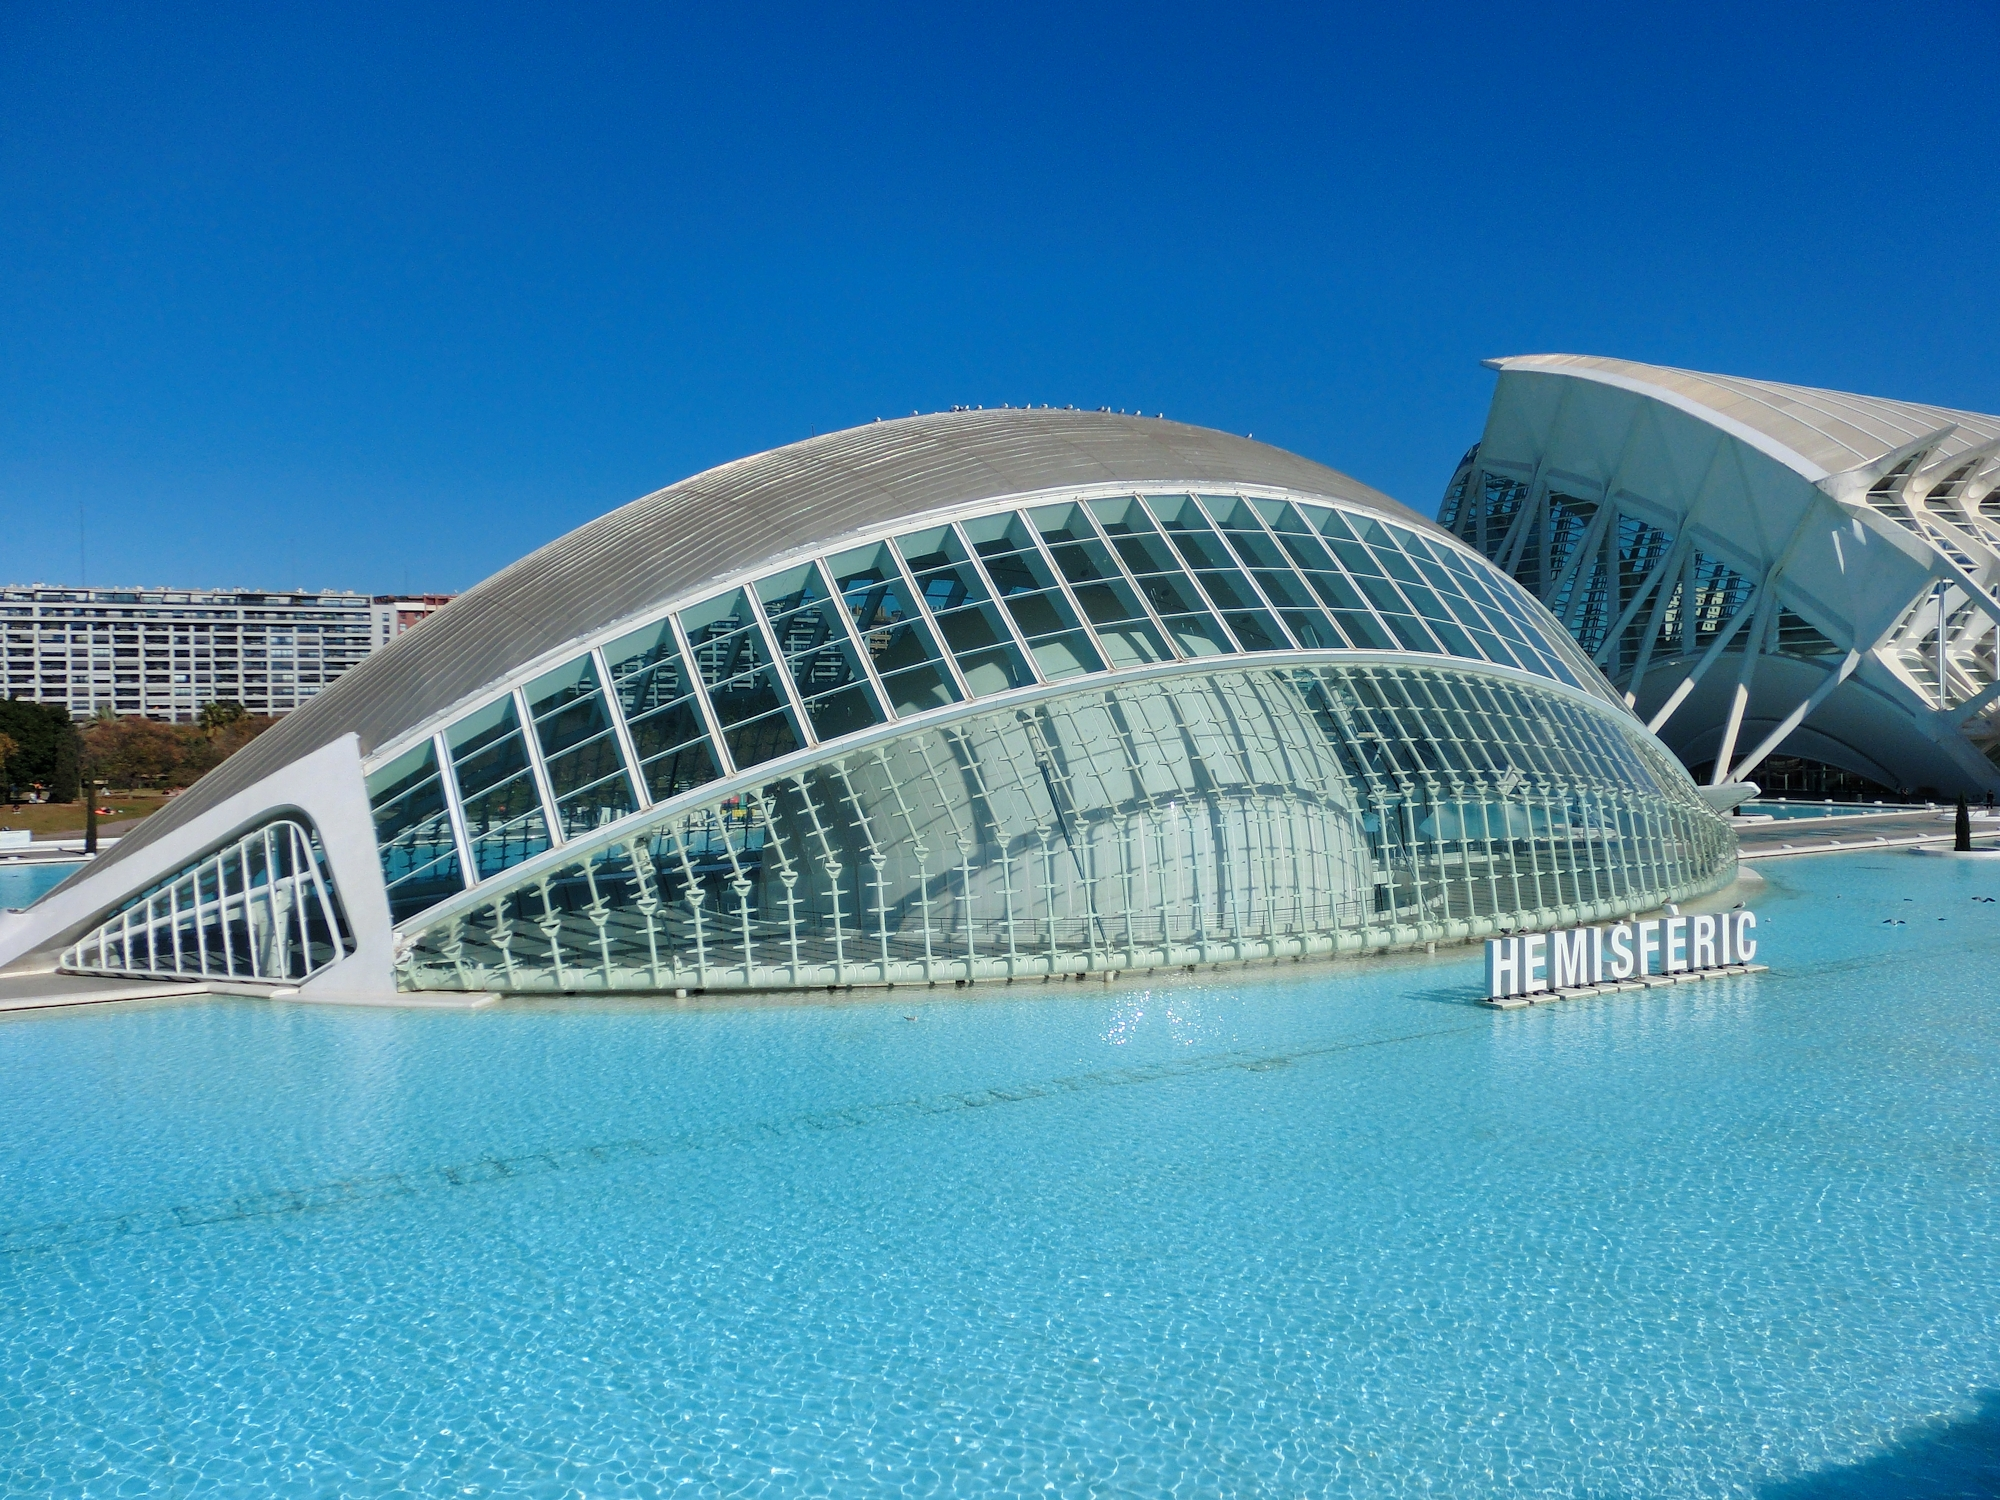
\includegraphics[height=\paperheight,width=\paperwidth]{hemisferic.jpg}};}
\begin{frame}
%\vspace{-20mm}
\maketitle
\end{frame}}
%\begin{frame}
%\maketitle
%\end{frame}

\section{Introduction}

\begin{frame}{Gabriel likes (to propose) problems}
%\onslide<1->{ \phantom{text}}
\begin{itemize}%[<+->]
%Zitate, Annals paper
\item<2-> 1994: \emph{Some Open Problems on Coprime Action and Character Correspondences}, Bull. London Math. Soc. 26, 513--522
\item<3-> 2004: \emph{Problems on characters and Sylow subgroups}, in: Finite groups, 275--281
\item<4-> 2010: \emph{Problems in character theory}, in: Character theory of finite groups, 97--125 %Contemp. Math. 524
\item<5-> 2023: \emph{Problems on characters: solvable groups}, Publ. Mat. 67, 173–198
\item<6-> 2024: \alert{“All I would like to prove has been proved!”}, e-mail correspondence %. But it is difficult to quit
\end{itemize}
\end{frame}

\section{Groups}
\begin{frame}{Automorphisms}
Let $G$ be a finite group.
\begin{Definition}[Automorphism tower]<2->
Let $\Aut^0(G):=G$ and $\Aut^{n+1}(G):=\Aut(\Aut^n(G))$ for $n\ge 0$. 
\end{Definition}
\onslide<3->{
If $\Z(G)=1$, then $G\cong\Inn(G)\le\Aut^1(G)\le\Aut^2(G)\le\ldots$.}

\begin{Theorem}[\textsc{Wielandt}]<4->
If $\Z(G)=1$, then $\Aut^n(G)\cong \Aut^{n+1}(G)$ for some $n$.
\end{Theorem}
\end{frame}

\begin{frame}{Automorphisms}

\begin{Theorem}[\textsc{Hamkins}]<+->
The transfinite automorphism tower of any group is bounded by some cardinal number.
\end{Theorem} 

\begin{Problem}[(Kourovka notebook 11.123)]<+->%Scott S. 457
\begin{itemize}
\item Is there a constant $c$ such that $|\Aut^n(G)|<c$ for all $n$?
\item Is $\Aut^n(G)\cong \Aut^{n+1}(G)$ for some $n$?
\item Can $\Aut^n(G)\cong \Aut^{m}(G)\not\cong \Aut^{n+1}(G)$ happen form some $n<m$? %Smith, 1964? Thomas Question 5.2.5
\end{itemize}
\end{Problem}

\end{frame}

\begin{frame}{Examples}
\begin{Example}
\begin{itemize}[<+->]
\item If $G$ is non-abelian simple, then $\Aut^2(G)\cong\Aut(G)$ (\textsc{Burnside}).
\item $\Aut(C_2^n)\cong\GL(n,2)$ is simple (for $n\ge 3$), so $\Aut^3(C_2^n)\cong\Aut^2(C_2^n)$. 
\item $\Aut(D_8)\cong D_8$. 
%\item Dickson's conjecture: There exist arbitrarily long sequences of primes $(p_1,\ldots,p_n)$ such that $p_{k+1}=2p_k+1$ for $k=1,\ldots,n-1$. Then
%$\Aut^k(C_{p_n})\cong C_{2p_{n-k}}$ for $k=1,\ldots,n-1$. 
\item The sequence can decrease arbitrarily long: $\Aut(C_{2\cdot 3^n})\cong C_{2\cdot 3^{n-1}}$  %https://oeis.org/A117729
%\[G=C_{2\cdot 3^n}\xrightarrow{\Aut}C_{2\cdot 3^{n-1}}
%\item It can go up and down: $C_8\xrightarrow{\Aut}C_2^2\xrightarrow{\Aut}S_3$.
\item For $G=\mathtt{SmallGroup}(32,13)$ we have 
\[\begin{array}{c|cccccc}
n&0&1&2&3&4&5\\\hline
\vphantom{M^{M^M}}
|\Aut^n(G)|&2^5&2^7&2^{13}&2^{28}&2^{83}&?
\end{array}\]
%
%$|\Aut(G)|=2^7$, $|\Aut^2(G)|=2^{10}$, $|\Aut^3(G)|=2^{18}$, $|\Aut^4(G)|=2^{49}$, $|\Aut^5(G)|=?$.
\end{itemize}
\end{Example}
\end{frame}

\begin{frame}{Homomorphisms}
\begin{Theorem}[\textsc{Frobenius}]<+->
For every $n$, the number of $x\in G$ such that $x^n=1$ is divisible by $\gcd(n,|G|)$. 
%\[|\{x\in G:x^n=1\}|\equiv 0\pmod{\gcd(n,|G|)}.\]
\end{Theorem}
\onslide<+->{
Equivalently,
\[|\Hom(C_n,G)|\equiv 0\pmod{\gcd(n,|G|)}.\]}
\begin{Theorem}[\textsc{Yoshida}]<+->
For every finite abelian group $A$,
\[|\Hom(A,G)|\equiv 0\pmod{\gcd(|A|,|G|)}.\]
\end{Theorem}

\end{frame}

\begin{frame}{Homomorphisms}
\begin{Con}[(\textsc{Asai-Yoshida})]<+->
For every finite group $H$,
\[|\Hom(H,G)|\equiv 0\pmod{\gcd(|H/H'|,|G|)}.\]
\end{Con}
\end{frame}

%\section{Conjugacy classes}
\begin{frame}{Conjugacy classes}
\begin{itemize}[<+->]
\item Let $k(G)$ be the number of conjugacy classes of $G$.

\item \textsc{Landau}: $k(G)>f(|G|)$ for some monotone function $f$.
\end{itemize}
%\onslide<+->{
%Let $k(G)$ be the number of conjugacy classes of $G$.}\\
%\onslide<+->{
% }

\begin{Theorem}[\textsc{Baumeister--Maróti--Tong-Viet}]<+->%\log2??
For every $\epsilon>0$ there exists $\delta>0$ such that
\[k(G)>\frac{\delta\log|G|}{(\log\log|G|)^{3+\epsilon}}.\]
\end{Theorem}

\begin{Con}[(Folklore?)]<+->
Is there a constant $c$ such that $k(G)>c\log|G|$?
\end{Con}
\end{frame}

%\begin{frame}{Conjugacy classes}
%\begin{Con}[(\textsc{Pyber})]%Kourovka 14.74
%Let $S_p\in\Syl_p(G)$ for a prime $p$. Then $k(G)\le\prod_pk(S_p)$.
%\end{Con}
%
%\begin{Con}[(\textsc{Liebeck--Pyber})]%Kourovka 14.54, solvable exists
%Is there a nilpotent subgroup $N\le G$ such that $k(G)\le|N|$?
%\end{Con}
%\end{frame}

\section{Characters}

\begin{frame}{Constituents}
\onslide<+->{
Let $\Irr(G)$ be the set of irreducible complex characters of $G$.}

\begin{Con}[(\textsc{H\'ethelyi--Külshammer})]<+->
Let $P$ be a $p$-group and $\chi\in\Irr(P)$. Then the number of irreducible constituents of $\chi\overline{\chi}$ is $1$ mod $p-1$. 
\end{Con}
\onslide<+->{
Conjecture holds for $|P|\le p^6$.
}

\begin{Problem}[(\textsc{Knutson--Murray})]<+->%Knutson p.104
Let $P$ be a $p$-group and $\chi\in\Irr(P)$. Is there a generalized character $\psi$ such that $\chi\psi$ is the regular character of $P$?
\end{Problem}
%use "new" integer linear programming
\end{frame}

%\begin{frame}
%\begin{Con}[\textsc{Harada}]
%\[\prod_{\chi\in\Irr(G)}\chi(1)\text{ divides }\prod_{K\in\Cl(G)}|K|.\]
%\end{Con}
%\end{frame}

\begin{frame}{Constituents}
%\begin{itemize}[<+->]
%%\item Let $N\unlhd G$ and $\theta\in\Irr(G)$ be $G$-invariant. 
%\item Call $\theta\in\Irr(\Z(G))$ \alert{fully ramified} if $\chi^G$ is a multiple of an irreducible character.
%\end{itemize}
\onslide<+->{Call $\theta\in\Irr(\Z(G))$ \alert{fully ramified} if $\chi^G$ is a multiple of an irreducible character.}
\begin{Theorem}[\textsc{Howlett--Isaacs}]<+->
If $\theta\in\Irr(\Z(G))$ is fully ramified, then $G$ is solvable.
\end{Theorem}
\begin{Con}[(\textsc{Humphreys}, \textsc{Navarro})]<+->
Let $\theta\in\Irr(\Z(G))$ such that all constituents of $\theta^G$ have the same degree. Then $G$ is solvable.
\end{Con}
\onslide<+->{Conjecture holds whenever $\theta^G$ has at most two constituents (\textsc{Higgs}).}
\end{frame}

\begin{frame}{Field of values}
\onslide<+->{
For $\chi\in\Irr(G)$ define the abelian number fields
\begin{align*}
\QQ(\chi)&:=\QQ\bigl(\chi(g):g\in G\bigr)\subseteq \QQ_{|G|}\subseteq\CC,\\
\QQ(G)&:=\QQ\bigl(\chi(g):\chi\in\Irr(G),\ g\in G\bigr)\subseteq \QQ_{|G|}.
\end{align*}}%
\onslide<+->{%
By the \textsc{Kronecker--Weber} theorem, every abelian number field lies in some $\QQ_n$. }

\begin{Theorem}[\textsc{Fein--Gordon}]<+->
For every abelian number field $F$ there exist a group $G$ and $\chi\in\Irr(G)$ such that $\QQ(\chi)=F$. 
\end{Theorem}

\end{frame}

\begin{frame}{Field of values}
\begin{Con}
\begin{itemize}[<+->]
\item Not every abelian number field has the form $\QQ(G)$.
\item For every $d$, there are only finitely many number fields $\QQ(G)$ of degree $d$.
\end{itemize}
\end{Con}
\onslide<+->{%
There are only finitely many fields $\QQ(G)$ of degree $d$ where $G$ is solvable or simple (\textsc{Farias e Soares}, \textsc{Feit--Seitz}).}

\begin{example}[quadratic fields]<+->
Let $d\mid 210$ or $d\in\{-231,-11,13,17\}$. Then there exists $G$ with $\QQ(G)\cong\QQ(\sqrt{d})$. 
\end{example}

\end{frame}

\begin{frame}{Field of values}
\begin{Theorem}[\textsc{Robinson--Thompson}]<+-> %gives all elementary abelian 2-groups
For $n>24$ we have
\[\QQ(A_n)=\QQ\Bigl(\sqrt{(-1)^{\frac{p-1}{2}}p}:p\text{ odd prime }\le n,\ p\ne n-2\Bigr).\]
In particular, $\Gal(\QQ(A_n)|\QQ)$ is an elementary abelian $2$-group.
\end{Theorem}
\begin{Problem}<+->
\begin{itemize}[<+->]
\item Is every abelian group the Galois group of some $\QQ(G)$? %relation??
\item Is there a group $G$ such that $|\QQ(G):\QQ|=7$?
\item Is there a group $G$ such that $\QQ(G)=\QQ(\sqrt{11})$?
\item Is there a solvable group $G$ such that $\QQ(G)=\QQ(\sqrt{-5})$?
%\item Are there rational groups with composition factor $C_7$ or $C_{11}$ (\textsc{Thompson})?
\end{itemize}
\end{Problem}

\end{frame}

\begin{frame}{Field of values}
\onslide<+->{
For $\chi\in\Irr(G)$ let $f(\chi)$ be the smallest integer $n$ such that $\QQ(\chi)\subseteq\QQ_n$. }

\begin{Con}[(\textsc{Hung--Tiep})]<+->
We have $|\QQ_{f(\chi)}:\QQ(\chi)|\le\chi(1)$ for all $\chi\in\Irr(G)$.
\end{Con}
\onslide<+->{Conjecture holds whenever $\chi(1)$ is a prime.}
\begin{Problem}[(\textsc{Hung--Tiep})]<+->
Let $z=\zeta_1+\ldots+\zeta_n\in\CC$ be a sum of roots of unity. Let $c(z)$ be the smallest $n$ such that $z\in\QQ_n$. Is $|\QQ_{c(z)}:\QQ(z)|\le n$?
\end{Problem}

\end{frame}

\begin{frame}{Algebraic integers}
\begin{itemize}[<+->]
\item Let $\ZZ_G$ be the ring of integers of $\QQ(G)$.
\item Let $\ZZ[G]:=\ZZ[\chi(g):\chi\in\Irr(G),\ g\in G]\subseteq\ZZ_G$. 
\item Then $\ZZ_G/\ZZ[G]$ is a finite abelian group.
\end{itemize}

\begin{Con}[(\textsc{Bächle--S.})]<+->
The exponent of $\ZZ_G/\ZZ[G]$ divides $|G|$.
\end{Con}

\begin{Example}<+->
Conjecture hold for nilpotent groups. For $G= C_{15}\rtimes D_{16}$, 
\[ \ZZ_G/\ZZ[G]\cong C_{120}^2\times C_{60}^2\times C_{12}^4\times C_4^4\times C_2^{14}.\]
\end{Example}

\end{frame}

\begin{frame}{Weights}
\begin{itemize}[<+->]
\item Let $\pi$ be a set of primes.
\item Let $l(G)$ be the number of conjugacy classes of $\pi'$-elements of $G$.
\item Let $\chi\in\Irr(G)$ of $\pi$-\alert{defect} $0$ if $|G|/\chi(1)$ is a $\pi'$-number.
\item Let $k^0(G)$ be the number of $\pi$-defect $0$ characters of $G$.
\end{itemize}

\begin{Theorem}[\textsc{Navarro--S.}]<+->
If $G$ is $\pi$-separable with solvable Hall $\pi$-subgroups, then
\[l(G)=\sum_{P}k^0(\N_G(P)/P)\]
where $P$ runs through the nilpotent $\pi$-subgroups of $G$ up to conjugation.
\end{Theorem}
\end{frame}

\begin{frame}{Weights}
\begin{itemize}[<+->]
\item For $\pi=\{p\}$, this becomes Alperin's weight conjecture for $p$-solvable groups. 

\item If the Hall subgroups are not solvable, we conjecture the following.
\end{itemize}

\begin{Con}[(\textsc{Navarro--S.})]<3->
Every group $P$ has a uniquely determined \alert{weight} $w(P)\in\ZZ$ such that for every $\pi$-separable group $G$, 
\[l(G)=\sum_{P}w(P)k_0(\N_G(P)/P)\]
where $P$ runs through the $\pi$-subgroups of $G$ up to conjugation.
\end{Con}

\end{frame}

\begin{frame}{Weights}
\begin{itemize}[<+->]
\item If $\pi$ is the set of prime divisors of $|P|$, then $P$ is $\pi$-separable and
\[w(P)=1-\sum_{\substack{Q<P\\\N_P(Q)=Q}}w(Q).\]
\item If $P$ is nilpotent, then $w(P)=1$. If $P$ is solvable, but not nilpotent, then $w(P)=0$ (\textsc{Carter} subgroups).
%\item $G$ contains at most one self-normalizing nilpotent subgroup (\textsc{Carter}, \textsc{Vdovin}).
\item On the other hand, %$w(P)=w(P/\Z(P))$
\[\begin{array}{c|ccccccc}
P&A_5&A_6&A_7&A_8&\PSL(3,4)&A_5^2&S_n(3\le n\le 11)\\\hline
w(P)&1&-2&1&-1&6&-1&0
\end{array}\]
\end{itemize}
\end{frame}

\section{Blocks}
\begin{frame}{Blocks}
\onslide<+->{Let $G^0$ be the set of $p$-regular elements of $G$.}
\begin{Theorem}[\textsc{Osima}]<+->
If $J\subseteq\Irr(G)$ such that
\[\sum_{\chi\in J}\chi(g)\chi(h)=0\qquad(\forall g\in G^0,\ h\in G\setminus G^0),\]
then $J$ is a union of blocks.
\end{Theorem}

\begin{Con}[(\textsc{Harada})]<+->
It is enough to fix $g=1$ in Osima's theorem.
%If $\varnothing \ne J\subseteq\Irr(B)$ such that
%\[\sum_{\chi\in J}\chi(1)\chi(g)=0\qquad(\forall g\in G\setminus G^0),\]
%then $J=\Irr(B)$.
\end{Con}
\end{frame}

\begin{frame}{Blocks}
\begin{itemize}[<+->]
\item Let $B$ be a $p$-block of $G$.
\item For $\chi\in\Irr(G)$ let $\chi^0$ be the restriction to $G^0$.
\item The Brauer characters in $p$-solvable groups have the form $\chi^0$ (\textsc{Fong--Swan}).
\end{itemize}
\begin{Con}[(ordinary basic set, \textsc{Geck})]<+->
There exist $\chi_1,\ldots,\chi_l\in\Irr(B)$ such that $\chi_1^0,\ldots,\chi_l^0$ is a basis of the Grothendieck group $\ZZ\IBr(B)$ of generalized Brauer characters. 
\end{Con}
\end{frame}

\begin{frame}{Blocks}
\begin{itemize}[<+->]
\item For $\chi,\psi\in\Irr(G)$ let
\[[\chi,\psi]^0=\frac{1}{|G|}\sum_{g\in G^0}\chi(g)\overline{\psi(g)}.\]

\item Let $d$ be the defect of $B$. Then $p^d[\chi,\chi]^0\in\NN$ for all $\chi\in\Irr(B)$.
\end{itemize}
\begin{Con}[(\textsc{Navarro-S.})]<+->
We have $l(B)\le p^d[\chi,\chi]^0$ for all $\chi\in\Irr(B)$. 
\end{Con}
\begin{itemize}[<+->]
\item This implies Brauer's conjecture $k(G)\le p^d$ with equality only if $B$ has abelian defect groups.

\item The case $\chi=1_G$ was conjectured by \textsc{Murai} and implies \textsc{Frobenius} conjecture: $G$ is $p$-nilpotent iff $|G^0|=|G|_{p'}$ (known via CSFG).
\end{itemize}
%For the principal block and $\chi=1_G$, this was conjectured by Murai. 
\end{frame}

%\begin{frame}{Matrices}
%\onslide<+->{
%The Cartan matrix of $B$ is indecomposable, i.\,e. not of the form $\begin{sm}
%*&0\\0&*
%\end{sm}$. }
%
%\begin{Con}[(\textsc{S.})]<+->
%If $C\in\ZZ^{l\times l}$ is the Cartan matrix of a block and $S\in\GL(l,\ZZ)$, then $SCS^{-1}$ is indecomposable.
%\end{Con}
%\end{frame}

\begin{frame}{Fusion number}
\begin{itemize}[<+->]
\item Let 
\[X_B:=\bigl(\chi(g_i):\chi\in\Irr(B),\ i=1,\ldots,k(G)\bigr)\] 
be a submatrix of the character table. 

\item The non-zero elementary divisors of $X_B^\TT\overline{X_B}$ over a complete discrete valuation ring are $p$-powers $e_1,\ldots,e_t$.
\end{itemize}
 
\begin{Con}[(\textsc{S.})]<+->
We have $\gamma(B):=\frac{1}{e_1}+\ldots+\frac{1}{e_t}\ge 1$ with equality if and only if $B$ is nilpotent.
\end{Con}
\begin{example}<+->
Conjecture holds for symmetric groups and “ATLAS groups”. For the principal $2$-block $B$ of the Monster, $\gamma(B)\approx 39.5$. %Lie type in def char
\end{example}
\end{frame}


\begin{frame}{Some memories}
\begin{itemize}[<+->]
\item \emph{I read your question just before going to bed and you have ruined my night. Good question. I dreamt that I had an example. }
%I will try to reconstruct now.

\item \emph{I am two days, 18 hours each,  trying to clean up the inductive McKay, no waving hands.} {\small [finishing his second book]}

\item \emph{If these two guys are not Morita equivalent then I won't say the word Morita again!} {\small [they weren't]}

%\item \emph{I have been dreaming tonight that we had a counterexample...}

%\item 04:38: \emph{OK, I am reading now (a bit early).}

\item \emph{Silly? I am in the middle of a restaurant.}

\item \emph{Seriously, I have thought on this for 3 minutes.}

\item \emph{Zero} {\small [answer to: How many examples did you check?]}

%\item \emph{I already had the title for our landmark paper : “A Jordan-Holder theorem for characters”!}

%\item \emph{We are really wasting time, but it is fun!}

%\item \emph{I won't be working except with my head and the iphone}

\item \emph{I am also amazed by my intuition, sorry to say!}

%\item \emph{I’m still recovering from the other problem. We do have learned. (I am also amazed by my intuition, sorry to say!)}

\item \emph{25th anniversary of my wedding. I have promised my wife not to think on mathematics for a couple of days. Now you are making my promise easy to break…}

%I am about to go: 25th anniversary of my wedding. I have promised
%my wife not to think on mathematics for a couple of days.
%Now you are making my promise easy to break...
\end{itemize}

\end{frame}

\end{document}

Title: Things left to prove
Abstract: I present some less-known open problems on groups, characters and blocks.

- Feit's conjecture on field of values
Ellers' conjecture (refinement of AWC)
- Eveev's conjecture

k(B)\le \rho(C) for p-solvable groups (Wada)
k(GV)\le |G|_p|V|
p-base conjecture, connection with some Navarro conjecture?
Where is his ironic review?

03.12.17: I read your question just before going to bed and you have
ruined my night. Good question. I dreamt that I had an example.
I will try to reconstruct now

18.08.17: I am two days, 18 hours each,  trying to clean up the inductive McKay, no waving hands. (heading towards his second book)

22.03.17: If these two guys are not Morita equivalent then I won't say the word Morita again!

22.03.17 03:08: I have been dreaming tonight that we had a counterexample...

16.09.15 04:38: OK, I am reading now (a bit early).


